\chapter{Guide for New Users}

\newcommand{\netcdf}{NetCDF}

%%%%%%%%%%%%%%%%%%%%%%%%%%%%%%%%%%%%%%%%%%%%%%%
% Progression Bar
% |==============>   |
% empty chapter        chapter finished
%%%%%%%%%%%%%%%%%%%%%%%%%%%%%%%%%%%%%%%%%%%%%%%

This tutorial is meant for people with some knowledge and/or experience in modelling and Linux, but which have no experience with the ICON model. In the following we will describe in short how to compile and run ICON on your machine. 

\section{Needed Software}

For some components ICON uses external libraries. Therefore you will need some additional software which should be installed on your machine. The following software needed to be installed on your machine:

\begin{itemize}
 \item \netcdf : \netcdf is a set of software libraries and self-describing, machine-independent data formats that support the creation, access, and sharing of array-oriented scientific data.\newline
 (Source: \href{http://www.unidata.ucar.edu/software/netcdf/}{http://www.unidata.ucar.edu/software/netcdf/})
 \item GRIB: GRIB (GRIdded Binary) is a format defined by the WMO (World Meteorological Organization). The use of GRIB in ICON is optional. The ECMWF GRIB API is an application program interface accessible from C, FORTRAN and Python programs developed for encoding and decoding WMO FM-92 GRIB edition 1 and edition 2 messages. A useful set of command line tools is also provided to give quick access to GRIB messages. ICON requires GRIB2 format. \newline
 (Source: \href{https://software.ecmwf.int/wiki/display/GRIB/Home}{https://software.ecmwf.int/wiki/display/GRIB/Home})
 \item MPI: MPI is a library specification for message-passing, proposed as a standard by a broadly based committee of vendors, implementors, and users.\newline
 (Source: \href{http://www.mcs.anl.gov/research/projects/mpi/}{http://www.mcs.anl.gov/research/projects/mpi/})
 \item OpenMP: Jointly defined by a group of major computer hardware and software vendors, the OpenMP API is a portable, scalable model that gives shared-memory parallel programmers a simple and flexible interface for developing parallel applications on platforms ranging from embedded systems and accelerator devices to multicore systems and shared-memory systems.\newline
 (Source: \href{http://openmp.org/wp/}{http://openmp.org/wp/})
\end{itemize}

\section{The Source Code}
% Filenames and URL needs to be adapted
You can obtain the source code on the website of DKRZ:

\href{https://www.dkrz.de/}{https://www.dkrz.de/}

You can use the following commands to untar the ICON source code:

\begin{verbatim}
tar xfvz icon.tar.gz
\end{verbatim}

This will create a folder \verb+icon-1.0+ inside your current directory. Within the ICON User Guide, this folder will further on be called \verb+$ICONDIR+.

\subsection{Directory structure}

Within \verb+$ICONDIR+, you will find a set of subdirectories. The important subdirectories are described in the following. 

\subsubsection{build}

Within the \verb+$ICONDIR/build+ directory, a subdirectory with the name of your computer architecture is created at compilation. Within this subdirectory, a \verb+bin+ subdirectory containing the binary \verb+control_model+ and several further subdirectories containing the compiled module files are created at compilation. 

\subsubsection{config}

Inside the \verb+$ICONDIR/config+ directory, different machine dependent configuration are stored within the configuration files. You can find a description of how to use and set up such configuration files in chapter \ref{chap:UG_config_compil}.

\subsubsection{data}

Within the \verb+$ICONDIR/data+ directory, you will find divers input datasets. For example, there are the datasets \verb+"rrtmg_lw.nc"+ and \verb+"ECHAM6_CldOptProps.nc"+, which are necessary for the radiation scheme (see sec. \ref{InputReal:Rad}). 

\subsubsection{doc}

Within the \verb+$ICONDIR/doc+ directory, several documentations for ICON are stored. There are according subdirectories for scientific (\verb+$ICONDIR/doc/science+), technical (\verb+$ICONDIR/doc/technical+) and programming style guides (\verb+$ICONDIR/doc/style+).

\subsubsection{externals}

Within the \verb+$ICONDIR/externals+ directory, external libraries for ICON are stored. Currently, it is the mtime library which is used to convert different date time formats.

\subsubsection{include}

Within the \verb+$ICONDIR/include+ directory, interfaces to libraries needed by ICON are stored. Currently, the interface to the CDI library is stored inside this directory. 

\subsubsection{run}

Within the \verb+$ICONDIR/run+ directory, namelist descriptor files as well as the full namelist documentation are stored. The namelist descriptor files can be used to generate runscripts. Further information can be found in \ref{chap:UG_running_model}.

\subsubsection{src}

Within the \verb+$ICONDIR/src+ directory, the source code of ICON including the main program and ICON modules can be found. The modules are ordered in several subdirectories which are described in the following. 

The main program \verb+control_model.f90+ can be found inside the subdirectory \newline \verb+$ICONDIR/src/drivers+. Additionally, this directory contains the modules for a hydrostatic and a nonhydrostatic setup.

The configuration of an ICON run is performed within the modules inside \newline \verb+$ICONDIR/src/configure_model+ and \verb+$ICONDIR/src/namelists+. Modules regarding the configuration of idealized test cases can be found inside \verb+$ICONDIR/src/testcases+.

The dynamics of ICON are inside \verb+$ICONDIR/src/atm_dyn_iconam+ and the physical parameterizations inside \verb+$ICONDIR/src/atm_phy_nwp+. Parameterizations for the interactions with the surface can be found inside \verb+$ICONDIR/src/lnd_phy_nwp+.

Shared infrastructure modules for 3-D and 4-D variables can be found within \newline \verb+$ICONDIR/src/shared+. The according routines for 2-D fields (e.g. external parameters) are stored within \verb+$ICONDIR/src/shr_horizontal+.

Modules handling the parallelization can be found in \newline\verb+$ICONDIR/src/parallel_infrastructure+.

Input and output modules are stored in \verb+$ICONDIR/src/io+.

The modules for the grid generator, as described in chapter \ref{chap:UG_grid_generation} can be found inside \newline \verb+$ICONDIR/src/grid_generator+.

\subsubsection{support}

Within the \verb+$ICONDIR/support+ directory, the CDI library is stored. 

\subsubsection{vertical\_coord\_table}

Inside the \verb+$ICONDIR/vertical_coord_tables+ directory, information files describing the relation between model layer, pressure and height are stored.

\section{Configuration and Compilation}
\label{chap:UG_config_compil}

%Configure and Compile

To ease up the compilation a configure-file is provided which should take over the main work. This Autoconf configuration is used to analyze the computer architecture (hardware and software) and set user specified preferences, e.g. the compiler. This preferences are read from \verb+config/mh-<OS>+, where \verb+<OS>+ is the identified operating system. Operating systems are listed in the configure-files in \verb+$ICONDIR/config/+ with the according files \verb+mh-<OS>+. If your machine is not listed you can add a config-file with your own \verb+<OS>+ based on the given \verb+mh-<OS>+ files. If different compilers are available, the \verb+mh-<OS>+ file may contain a case construct to distinguish them. If your \verb+<OS>+ is not recognized but is one of the listed \verb+<OS>+ you can invoke the configure file with the according option \verb+--host=$HOST+. Examples for the DWD CRAY system are given in the boxes.

\subsection{Description of the Configuration Files}

To add a specific compiler or change your compiler flags, you have to enter the \newline \verb+$ICONDIR/config/mh-<OS>+ according to your operating system \verb+<OS>+. For the DWD CRAY, the compiler flags in \verb+mh-linux+ look like the following:

\begin{Verbatim}[frame=single]
CRAY EXAMPLE: Compiler Flags inside mh-linux
cray)
    config_compiler=cray
	CC          = cc
    FC          = ftn
    F77         = "$FC"
    FFLAGS      = -v -D__LOOP_EXCHANGE -D__MIXED_PRECISION -Df2cFortran 
-e Z -em -hflex_mp=conservative -hfp1 -hadd_paren -r am -Ktrap=divz,ovf
    CFLAGS      = -I${GRIB_API}/include -v -Df2cFortran 
-DHAVE_CF_INTERFACE -DHAVE_LIBNETCDF -DHAVE_LIBGRIB 
-DHAVE_LIBGRIB_API -O3  -D__SVN_VERSION="${SVNVERSION}"
    F77FLAGS    = "$FFLAGS"
    FCLIBS      = "-v"
    GEN_FLAGS   =
    FDEBUG      = -g -R abc
    OMPFLAG     = -mp
    DEFOPT      = -D
    DEFCOPT     = -D
    MODOPT      = -I
    MODDIR      = 
    ;;
\end{Verbatim}

The \verb+cray)+ in this example gives the name of this specific configuration. It can be addressed by a flag at configuration. For this example, the according command to choose this setting would be \verb+./configure --with-fortran=cray+ (see section \ref{sec:config_compile}). Like this, you can create your own configuration by adding a new compiler.

\verb+CC+, \verb+FC+ and \verb+F77+ are the compiler directives for C-Compiler, FORTRAN2003-Compiler and FORTRAN77-Compiler. The according compiler flags are set via \verb+CFLAGS+, \verb+FFLAGS+ and \verb+F77FLAGS+. The variable to set an OpenMP flag is called \verb+OMPFLAG+. Libraries are set via \verb+FCLIBS+. 

\subsection{Configuring and Compiling the Code} \label{sec:config_compile}

To configure the source code go to \verb+$ICONDIR+ and give:

\begin{small}
 \begin{verbatim}
  ./configure
  ./build_command
  \end{verbatim}
\end{small}

If you want to use another compiler than the default compiler you give:

\begin{small}
  \begin{verbatim}
   ./configure --with-fortran=<compiler>
   ./build_command
  \end{verbatim}
\end{small}

where \verb+<compiler>+ is \verb+{gcc,nag,intel,pgi,cray}+.

\begin{Verbatim}[frame=single]
CRAY EXAMPLE: Configure + Make
./configure --with-fortran=cray}
./build_command
\end{Verbatim}

Note, that CRAY compiler environment (cce) versions 8.2.x do not work with ICON. The CRAY configuration is expanded to the following:

\begin{Verbatim}[frame=single]
CRAY EXAMPLE: Configuration
ftn -I../module -v -D__LOOP_EXCHANGE -D__MIXED_PRECISION -Df2cFortran -e 
Z -em -hflex_mp=conservative -hfp1 -hadd_paren -r am -Ktrap=divz,ovf 
-D__ICON__ <object files> -L/usr/local/pkg/grib_api/1.11.0/CRAY/lib  
-L../lib -lsupport -lgrib_api_f90 -lgrib_api -lmtime $(LAPACK_LIB) 
$(NETCDF_LIB) $(HDF5_LIB) $(SZIP_LIB) $(ZLIB_LIB) $(MPI_LIB) 
$(METIS_LIB) $(PROFILE_LIB) $(SCT_LIB)
\end{Verbatim}

ICON is parallelized using MPI and OpenMP. You can control the parallelization to be used by giving:

\begin{small}
  \begin{verbatim}
   ./configure --with-mpi/--without-mpi --with-openmp/--without-openmp
   ./build_command
  \end{verbatim}
\end{small}

By default the options are set to \verb+--with-mpi --without-openmp+. After a successful build, you will find the ICON executable named \verb+control_model+ inside \verb+$ICONDIR/build/<OS>/bin/+. The CRAY Fortran compiler is an exception, as the command includes automatically OpenMP. Therefore, although selecting --without-openmp, OpenMP is used.

If you wish to re-configure ICON it is advisable first to clean the old setup by giving:

\begin{small}
  \begin{verbatim}
   make distclean  
  \end{verbatim}
\end{small}

Some more details on configure options can be found in the help of the configure command:

\begin{small}
 \begin{verbatim}
  ./configure --help
 \end{verbatim}
\end{small}

\section{Running the Model (Idealized Cases)}
\label{chap:UG_running_model_idealized}

To shed light on the functionality and the quality of the dynamical core, setups for two test cases are presented in the following. Additionally, results of these test cases are shown. These tests are classified in short deterministic test cases (typically a simulation period of about 10-30 days) and tests in a climate mode (typically a multi-year period). This section concentrates on the first class, which starts from prescribed initial conditions (ideally provided in analytic form). The simulation results are either compared to analytic solutions (if available) or high-resolution reference solutions. For a list of available testcases, the reader is referred to the namelist section (\ref{chap:namelists}).

\subsection{Jablonowski-Williamson test}

The Jablonowski-Williamson Test \citep{Jablonowski:2006} is a standard test for dynamical cores in global models and can be run for dry dynamics only - as it is intended for- but full physics can be also tested. 

Input von Daniel Reinert is expected here.

\subsubsection{Setup}

For full physics, two additional namelist parameters are introduced in the  \verb+testcase_nml+ to control the initial moisture in the atmosphere:
\begin{itemize}
\item Here \verb+rh_at_1000hpa+ to be set between $0$ and $1$. The default is set to $0.7$ which gives a quite smooth start. If you really want to see early onsets of convection and microphysics you have to tune this parameter.
\item \verb+qv_max+ is usually set to $20.e-3 kg/kg$ and refers to the maximum value in the tropics.
\end{itemize}

\subsubsection{Input Data}

GRID

\subsubsection{Results}

The \textbf{Jablonowski-Williamson steady-state test} is based on a zonally symmetric, strongly baroclinic atmosphere. Initially, it is in a hydrostatic and geostrophic balance and therefore should remain stationary if no perturbation is imposed. Grid irregularities can disturb this stationary conditions and hence the test identifies the presence and magnitude of grid imprinting of a numerical model.
For the \textbf{Jablonowski-Williamson baroclinic wave test}, a weak (and unbalanced) perturbation disturbs the initial wind. This test highlights the diffusivity (or effective resolution) of a dynamical core and the presence of phase speed errors in the advection of poorly resolved structures.

\subsection{Mountain induced Rossby waves}

In order to test the model dynamics in dry stage but with real or any complex topography one can choose the mountain induced Rossby wave test case and select different types of topography.



The following runfile gives an example how to perform such an idealized simulation.

\begin{landscape}

\begin{Verbatim}[frame=single]
NAMELIST EXAMPLE for a moutain induced Rossby waves

#! /bin/ksh
# ----------------------------------------------------------------------------
#PBS -q xc_normal
#PBS -l select=4:ompthreads=4
#PBS -l place=scatter
#PBS -l walltime=01:00:00
#PBS -j oe
#PBS -W umask=022
# ----------------------------------------------------------------------------
# ============================================================================
#
# Cray batch script for the ICON model
#
# Initializes the Jablonowski Williamson test case with a 
# mountain instead of the wind perturbation.
#
# Platform: Cray XC30
#           xce.dwd.de
#
# 05/2014 : F. Prill, DWD
#
# ----------------------------------------------------------------------------
# ============================================================================


set -x

# OpenMP settings
export OMP_SCHEDULE="static"
export OMP_DYNAMIC="false"
# MPI: use DMAPP for off-node data movement
export MPICH_RMA_OVER_DMAPP=1
# disable core dumps
export RLIMIT_CORE=0
export ATP_MAX_CORES=0


# ----------------------------------------------------------------------------
# path definitions
# ----------------------------------------------------------------------------

# directory with input grids:
GRIDDIR=/e/uhome/gzaengl/icon-dev/experiments/GRF_R2B4N6M

# base directory for ICON sources and binary:
ICONDIR=${PBS_O_WORKDIR}/../../

# absolute path to directory with plenty of space:
EXPDIR=/e/uhome/dreinert/icon/experiments/exp15_mrw

# path to model binary, including the executable:
MODEL=${ICONDIR}/build/x86_64-unknown-linux-gnu/bin/control_model


# ----------------------------------------------------------------------------
# copy input data: grids, external parameters
# ----------------------------------------------------------------------------

# the directory for the experiment will be created, if not already there
if [ ! -d $EXPDIR ]; then
    mkdir -p $EXPDIR
fi
cd ${EXPDIR}

ln -sf ${GRIDDIR}/iconR2B03_DOM00.nc iconR2B03_DOM00.nc
ln -sf ${GRIDDIR}/iconR2B04_DOM01.nc iconR2B04_DOM01.nc

# files needed for radiation
ln -sf ${ICONDIR}/data/ECHAM6_CldOptProps.nc .
ln -sf ${ICONDIR}/data/rrtmg_lw.nc .


# ----------------------------------------------------------------------------
# grid namelist settings
# ----------------------------------------------------------------------------

# the grid parameters
atmo_dyn_grids="iconR2B04_DOM01.nc"
atmo_rad_grids="iconR2B03_DOM00.nc"

# reconstruct the grid parameters in namelist form
dynamics_grid_filename=""
for gridfile in ${atmo_dyn_grids}; do
  dynamics_grid_filename="${dynamics_grid_filename} '${gridfile}',"
done
radiation_grid_filename=""
for gridfile in ${atmo_rad_grids}; do
  radiation_grid_filename="${radiation_grid_filename} '${gridfile}',"
done


# ----------------------------------------------------------------------------
# create ICON master namelist
# ----------------------------------------------------------------------------

cat > icon_master.namelist << EOF

! master_nml: ----------------------------------------------------------------
&master_nml
 lrestart                   =                      .FALSE.        ! .TRUE.=current experiment is resumed
/

! master_model_nml: repeated for each model ----------------------------------
&master_model_nml
 model_type                  =                          1         ! identifies which component to run (atmosphere,ocean,...)
 model_name                  =                      "ATMO"	  ! character string for naming this component.
 model_namelist_filename     =              "NAMELIST_NWP"	  ! file name containing the model namelists
 model_min_rank              =                          1	  ! start MPI rank for this model
 model_max_rank              =                      65536	  ! end MPI rank for this model
 model_inc_rank              =                          1         ! stride of MPI ranks
/

! time_nml: specification of date and time------------------------------------
&time_nml
 ini_datetime_string         =      "2011-01-01T00:00:00Z"        ! initial date and time of the simulation
/

EOF


# ----------------------------------------------------------------------------
# model namelists
# ----------------------------------------------------------------------------
# For a complete list see doc/Namelist_overview.pdf

cat > NAMELIST_NWP << EOF

! diffusion_nml: horizontal (numerical) diffusion ----------------------------
&diffusion_nml
 hdiff_order                 =                          5         ! order of nabla operator for diffusion
 itype_vn_diffu              =                          1	  ! reconstruction method used for Smagorinsky diffusion
 itype_t_diffu               =                          2	  ! discretization of temperature diffusion
 hdiff_efdt_ratio            =                         36.0	  ! ratio of e-folding time to time step 
 hdiff_smag_fac              =                          0.015	  ! scaling factor for Smagorinsky diffusion
 lhdiff_vn                   =                      .TRUE.	  ! diffusion on the horizontal wind field
 lhdiff_temp                 =                      .TRUE.	  ! diffusion on the temperature field
/

! dynamics_nml: dynamical core -----------------------------------------------
&dynamics_nml
 iequations                  =                          3	  ! type of equations and prognostic variables
 idiv_method                 =                          1	  ! method for divergence computation
 divavg_cntrwgt              =                          0.50	  ! weight of central cell for divergence averaging
 lcoriolis                   =                      .TRUE.	  ! Coriolis force
/

! extpar_nml: external data --------------------------------------------------
&extpar_nml
 extpar_filename             =                         ""         ! filename of external parameter input file
 itopo                       =                          0         ! topography (0:analytical)
/

! grid_nml: horizontal grid --------------------------------------------------
&grid_nml
 dynamics_grid_filename      =  ${dynamics_grid_filename}         ! array of the grid filenames for the dycore
 radiation_grid_filename     = ${radiation_grid_filename}         ! array of the grid filenames for the radiation model
 dynamics_parent_grid_id     =              0, 1, 2, 1, 4         ! array of the indexes of the parent grid filenames
 lredgrid_phys               = .TRUE.,.TRUE.,.TRUE.,.TRUE.,.TRUE. ! .true.=radiation is calculated on a reduced grid
 lfeedback                   =                      .TRUE.        ! specifies if feedback to parent grid is performed
 ifeedback_type              =                          2         ! feedback type (incremental/relaxation-based)
/

! gridref_nml: grid refinement and nesting -----------------------------------
&gridref_nml
 grf_intmethod_e             =                          6         ! interpolation method for grid refinement
 grf_scalfbk                 =                          2	  ! feedback method for dynamical scalar variables
 grf_tracfbk                 =                          2	  ! feedback method for tracer variables
 denom_diffu_v               =                        150.0	  ! Deniminator for lateral boundary diffusion of velocity
/

! io_nml: general switches for model I/O -------------------------------------
&io_nml
 dt_diag                     =                      21600.0       ! diagnostic integral output interval
 dt_checkpoint               =                    5760000.0       ! time interval for writing restart files.
 itype_pres_msl              =                          2         ! method for computation of mean sea level pressure
/

! nh_testcase_nml: idealized testcase specification --------------------------
&nh_testcase_nml
 nh_test_name                =                    'mrw_nh'        ! testcase selection
 u0_mrw                      =                       20.0         ! initial u-component of the wind velocity
 mount_height_mrw            =                     2000.0         ! maximum mountain height 
 mount_half_width            =                  1500000.0	      ! half width of mountain
 mount_longctr_mrw_deg       =                       90.0         ! longitude of the center of the mountain
 mount_latctr_mrw_deg        =                       30.0         ! latitude of the center of the mountain
/

! nonhydrostatic_nml: nonhydrostatic model -----------------------------------
&nonhydrostatic_nml
 ivctype                     =                          2	  ! type of vertical coordinate
 vwind_offctr                =                          0.2	  ! off-centering in vertical wind solver
 damp_height                 =                      50000.0	  ! height at which Rayleigh damping of vertical wind starts
 rayleigh_coeff              =                          0.10	  ! Rayleigh damping coefficient
 iadv_rcf                    =                          5	  ! calling frequency for transport/diffusion/physics
 lhdiff_rcf                  =                      .TRUE.	  ! .TRUE.=compute diffusion only at advection time steps
/

! output_nml: specifies an output stream --------------------------------------
&output_nml
 filetype                    =                          4         ! output format: 2=GRIB2, 4=NETCDFv2
 dom                         =                         -1         ! write all domains
 output_bounds               =       0., 10000000., 21600.        ! output: start, end, increment
 steps_per_file              =                          2         ! number of output steps in one output file
 mode                        =                          1         ! 1: forecast mode (relative t-axis), 2: climate mode (absolute t-axis)
 include_last                =                      .TRUE.        ! flag whether to include the last time step
 output_filename             =                       'NWP'        ! file name base
 output_grid                 =                      .TRUE.        ! flag whether grid information is added to output.
 !
 ml_varlist                  =  'u', 'v', 'w', 'temp', 'pres','topography_c', 'vor'
/

! parallel_nml: MPI parallelization -------------------------------------------
&parallel_nml
 nproma                      =                          8         ! loop chunk length
 p_test_run                  =                     .FALSE.	  ! .TRUE. means verification run for MPI parallelization
 num_io_procs                =                          1	  ! number of I/O processors
 num_restart_procs           =                          0	  ! number of restart processors
 iorder_sendrecv             =                          3         ! sequence of MPI send/receive calls
/

! run_nml: general switches ---------------------------------------------------
&run_nml
 ltestcase                   =                      .TRUE.	  ! idealized testcase runs
 num_lev                     =                         90         ! number of full levels (atm.) for each domain
 lvert_nest                  =                      .TRUE.        ! vertical nesting
 nsteps                      =                       1000         ! number of time steps of this run
 dtime                       =                        288         ! timestep in seconds
 ldynamics                   =                      .TRUE.        ! compute adiabatic dynamic tendencies
 ltransport                  =                      .FALSE.	  ! compute large-scale tracer transport
 ntracer                     =                          0	  ! number of advected tracers
 iforcing                    =                          0	  ! forcing of dynamics and transport by parameterized processes
 msg_level                   =                          7	  ! controls how much printout is written during runtime
 ltimer                      =                     .FALSE.	  ! timer for monitoring the runtime of specific routines
 output                      =                       "nml"        ! main switch for enabling/disabling components of the model output
/

! sleve_nml: vertical level specification -------------------------------------
&sleve_nml
 min_lay_thckn               =                         20.0       ! layer thickness of lowermost layer
 top_height                  =                      75000.0	  ! height of model top
 stretch_fac                 =                          0.9	  ! stretching factor to vary distribution of model levels
 decay_scale_1               =                       4000.0	  ! decay scale of large-scale topography component
 decay_scale_2               =                       2500.0	  ! decay scale of small-scale topography component
 decay_exp                   =                          1.2	  ! exponent of decay function
 flat_height                 =                      16000.0       ! height above which the coordinate surfaces are flat
/

EOF


# ----------------------------------------------------------------------------
# run the model!
# ----------------------------------------------------------------------------

cp -p $MODEL icon

# "aprun" command:
# -n xx   : number of MPI tasks
# -N xx   : number of MPI tasks/node
# -d  x   : number of threads/MPI task
# -j 2    : Hyperthreading enabled: 20 physical cores -> 40 "virtual" cores
# -m 3g   : 3G memory/task

aprun  -n 40 -N 10 -j 2 -d 4 -m 3g icon

\end{Verbatim}

\end{landscape}

\subsubsection{Initial conditions}

Applying this run file the topography shown in Fig. \ref{fig:mountain} is used.

\begin{figure}[h!]%
\centering
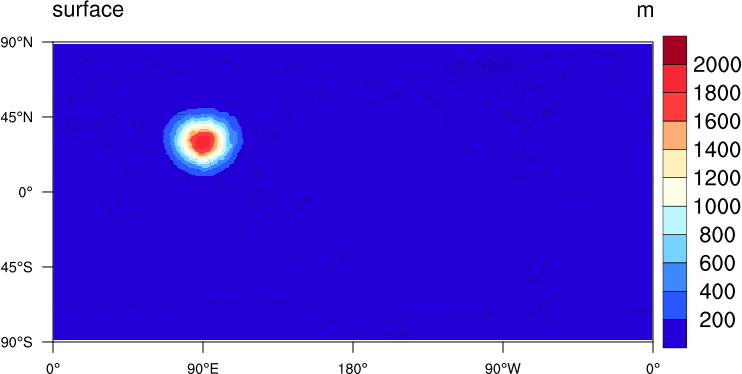
\includegraphics[width=0.95\linewidth]{pictures/surface-small.png}
\caption{Topography of the test case}\label{fig:mountain}
\end{figure}

The v-component of the wind speed is is initialized with zero at all grid points, the initial conditions for the u-component are shown in Fig. \ref{fig:u-initial}.

\begin{figure}[h!]%
\centering
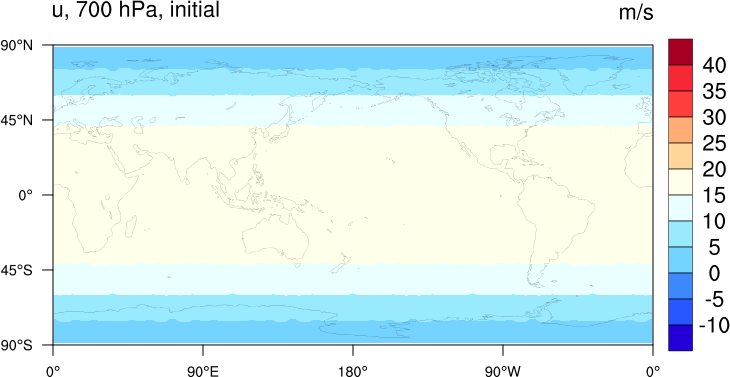
\includegraphics[width=0.95\linewidth]{pictures/u-initial-small.png}
\caption{Spatial distribution of the initialized u-component at 700 hPa}\label{fig:u-initial}
\end{figure}


This results in the spatial distribution of the initialized 
vorticity shown in Fig. \ref{fig:vorticity-initial}.

\begin{figure}[h!]%
\centering
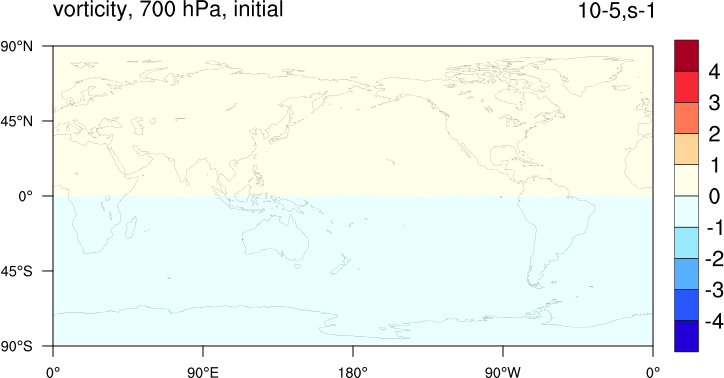
\includegraphics[width=0.95\linewidth]{pictures/vorticity-initial-small.png}
\caption{Spatial distribution of the initial conditions of the vorticity at 700 hPa}\label{fig:vorticity-initial}
\end{figure}

\subsubsection{Results after 16 days}



The u-component after sixteen days of simulation at 700 hPa is shown in Fig. \ref{fig:u-16}.

\begin{figure}[h!]%
\centering
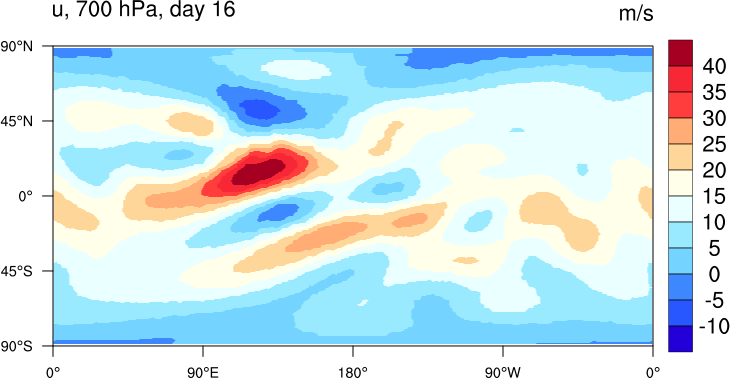
\includegraphics[width=0.95\linewidth]{pictures/u-day-16-small.png}
\caption{Spatial distribution of u-component after 16 days of simulation at 700 hPa}\label{fig:u-16}
\end{figure}


The spatial distribution of the initialized 
vorticity shown in Fig. \ref{fig:vorticity-16}.

\begin{figure}[h!]%
\centering
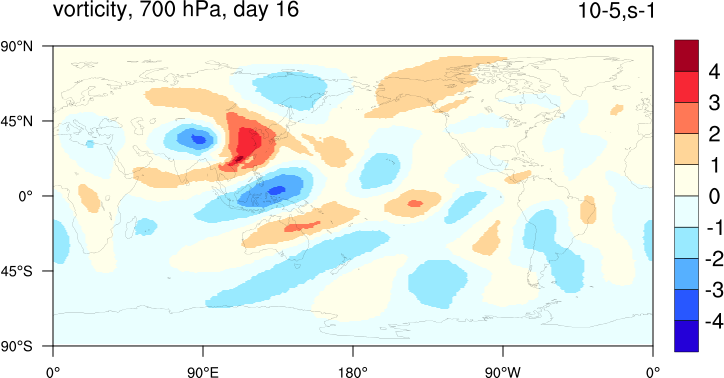
\includegraphics[width=0.95\linewidth]{pictures/vorticity-d16-small.png}
\caption{Spatial distribution of the vorticity after 16 days o simulation at 700 hPa}\label{fig:vorticity-16}
\end{figure}





\subsubsection{Input Data}

With the exception of the grid file no further input files are necessary. 




\section{Running the Model (Real Case)}
\label{chap:UG_running_model}


The ICON code, as checkout from the SVN repository, does not include runscripts. Instead the run directory (\verb+$ICONDIR/run/+) includes several descriptor files for building grids, defining experiments and post-processings. There exist three different types of descriptor files with prefixes \verb+grid, exp, post+:

\begin{itemize}
 \item \verb+grid.<name>+: to configure the grid generator, see chapter \ref{chap:UG_grid_generation} for more details. It is recommended to use pre-built grids. For details, see section \ref{chap:prebuilt_grid}.
 \item \verb+exp.<name>+: to define the namelist, which determinate the experiments.
 \item \verb+post.<name>+: to define post-processing.
\end{itemize}

\subsection{Input Data}

Generally ICON requires the following input data: Grid files, external parameters, initialization (DWD analysis or IFS), input fields for radiation.

\subsubsection{Grid Files}\label{sec:grid_input}

In order to run ICON, it is necessary to have the horizontal grid information as an input parameter. This information is stored within so-called grid files. For a ICON run, one global grid file is necessary. Additionally, if you want to nest, grid files of the nested domains are necessary, too. To improve the performance of ICON, a (optional) reduced radiation grid for each domain may be used. 

The naming of the ICON-Grid is as follows: The initial icosahedron grid is refined by \textless n\textgreater -secting the edges, and further refinement is obtained by iteratively bisecting the created edges. The grid produced at the \textless k\textgreater refining iteration is named "R\textless n\textgreater B\textless k\textgreater". For further details, see the ICON Technical Documentation.

It is recommended to use pre-built grids. Further information can be found in chapter \ref{chap:prebuilt_grid}. For building own grids, the reader is referred to chapter \ref{chap:UG_grid_generation}. The names of the grid files have to be specified within the \verb+grid_nml+:

\begin{verbatim}
&grid_nml
dynamics_grid_filename = "<INSERTFILENAME>"
radiation_grid_filename = "<INSERTFILENAME>"
\end{verbatim}

\subsubsection{External Parameters}\label{InputReal:Ext}

ICON requires geographical localized datasets like the topographic height of the earth surface, the plant cover, the distribution of land and sea and, dependent on the schemes used, a variety of other so called external parameters. The EXTPAR software system (EXTPAR - External Parameter for Numerical Weather Prediction and Climate Application) is able to generate external parameters for the different models GME, COSMO, HRM and ICON. The software can run on a UNIX or Linux systems where the raw data is stored. It allows operators (experienced users) running the scripts to create new external parameters controlled by user specifications like the model domain. For a more detailed overview of EXTPAR, the reader is referred to the User and Implementation Guide of EXTPAR. 

The name of the EXTPAR file which has to be read by ICON can be specified as follows:

\begin{verbatim}
&extpar_nml
extpar_filename = "<INSERTFILENAME>"
\end{verbatim}

If not specified explicitly, ICON uses the following file name: \newline
\verb+"<path>extpar_<gridfile>"+.\newline
 \verb+<path>+ and \verb+<gridfile>+ are then replaced at runtime by ICON.

\subsubsection{Initialization}\label{InputReal:Ini}

For the initialization of ICON, input data from either DWD or IFS is needed. 

In case of DWD (init\_mode=1) a first guess and an analysis is required: 
\begin{verbatim}
&initicon_nml
dwdfg_filename = "<INSERTFILENAME>"
dwdana_filename = "<INSERTFILENAME>"
\end{verbatim}

If not specified explicitly, ICON uses the following file names: \newline 
\verb+"<path>dwdFG_R<n>B<k>_DOM<idom>.nc"+ and \newline
\verb+"<path>dwdana_R<n>B<k>_DOM<idom>.nc"+. \newline
\verb+<path>+, \verb+<n>+, \verb+<k>+ and \verb+<idom>+ are then replaced at runtime by ICON according to the chosen gridfile (see \ref{sec:grid_input}). The variable \verb+<idom>+ is an index for the domain on which the calculations are performed. \verb+<idom>=0000+ is reserved for a reduced radiation grid, \verb+<idom>=0001+ for the global domain, higher numbers are used for nested domains. NETCDF as well as GRIB2 input can be used.

In case of IFS (init\_mode=2) an analysis is required. It has to be in \netcdf: 
\begin{verbatim}
&initicon_nml
ifs2icon_filename = "<INSERTFILENAME>"
\end{verbatim}

If not specified explicitly, ICON uses the following file name: \newline 
\verb+"<path>ifs2icon_R<n>B<k>_DOM<idom>.nc"+. \newline
\verb+<path>+, \verb+<n>+, \verb+<k>+ and \verb+<idom>+ are then replaced at runtime by ICON according to the chosen gridfile (see \ref{sec:grid_input}). The variable \verb+<idom>+ is an index for the domain on which the calculations are performed. \verb+<idom>=0000+ is reserved for a reduced radiation grid, \verb+<idom>=0001+ for the global domain, higher numbers are used for nested domains.

\subsubsection{Radiation}\label{InputReal:Rad}

ICON requires input fields for the RRTM radiation scheme. The file names are specified as follows:

\begin{verbatim}
&nwp_phy_nml
lrtm_filename = "<INSERTFILENAME>" 
cldopt_filename = "<INSERTFILENAME>"
\end{verbatim}

If not specified explicitly, ICON uses the following file names: \newline 
\verb+"rrtmg_lw.nc"+ and \newline
\verb+"ECHAM6_CldOptProps.nc"+.

The files can be found within \verb+$ICONDIR/data+.

\subsection{Creating a Runscript}

To create a runscript, new users are advised to use the namelist descriptor file \verb+exp.nh-oper+ which contains recently recommended namelist settings. It might be necessary to account for the file names and paths of the input data. Additionally, machine dependent settings need to be added to this script to obtain a runscript. For some architectures, this step can be performed by using the make runscript environment as shown in \ref{sec:make_runscript}. In the following, example settings for DWD CRAY are listed.

\begin{Verbatim}[frame=single]
CRAY EXAMPLE: Environment variables
#!/bin/ksh
#==============================================================
#PBS -q xc_normal
#PBS -l select=?:ncpus=?:mpiprocs=?:ompthreads=?:mem=?gb
#PBS -l place=scatter
#PBS -j oe
#PBS -N <<Jobname>>

export MPICH_RMA_OVER_DMAPP=1
\end{Verbatim}

\begin{Verbatim}[frame=single]
CRAY EXAMPLE: Namelists
<<Place your namelists e.g. from exp.nh_oper here>>
\end{Verbatim}

\begin{Verbatim}[frame=single]
CRAY EXAMPLE: Submitting a job
aprun                                    \
  -n <<INSERT: MPI Tasks>>            \
  -N <<INSERT: MPI Tasks/Node>>       \
  <<INSERT: Hyperthreading e.g. 2 -> 20 physical -> 40 "virtual" cores>> \
  -d <<INSERT: Threads/MPI Task>>     \
  -m <<INSERT: Amount of memory to use>> control_model
\end{Verbatim}


\subsection{Restart}

A restart of the model requires a restart file that has to be created by a 
previous model run. In the following the procedures and the corresponding namelist settings are explained.

\subsubsection{Creating the initial restart file:}

The first job in a series of model runs creates the first restart file.
To do so we have to use the following namelist switches.

\begin{verbatim}
&master_nml
lrestart = .FALSE. 
\end{verbatim}

In addition we have to prescribe at which time interval the job should produce a restart file:

\begin{verbatim}
&io_nml
dt_checkpoint = "<Insert time in seconds>" 
\end{verbatim}


The ICON run then creates restart files for each domain 1, ..., \verb+n_dom+, and for each restart
output time step. 

The filenames are generic and look like:

\begin{verbatim}
 "<gridfile>_restart_<modeltype>_<timestamp>.nc", 
\end{verbatim}

An example would be:

\begin{verbatim}
 "iconR2B06_DOM01_restart_atm_20110101T001200Z.nc"    (NetCDF format)
\end{verbatim}
   
This filename can be customized using the namelist parameter:
    
     
\begin{verbatim}
&mo_run_nml
restart_filename = "<INSERTFILENAME>" 
\end{verbatim}

This file contains:

\begin{itemize}
\item{data} 
\item{namelists}
\item{several attributes}
\end{itemize}


Note:
    -  ICON reads the namelists only once and assumes that these
       are identical for all domains.
    -  Since we do not know about the total number of domains at startup,
       we have to ask the current restart file for the attribute \verb+"n_dom"+.


For each domain 1, ..., \verb+n_dom+, a symbolic link is generated with the generic name: 

 \verb+"restart_<modeltype>_DOMxx.nc"+

     
     
 
Note:
    -  The domain-dependent suffix "...DOMxx" is also required for 
non-nested setups.

    


\subsubsection{Running the model in the restart mode:}

ICON has to be informed that you want to carry out a restart run:

\begin{verbatim}
&master_nml
lrestart = .TRUE. 
\end{verbatim}

The generic link \verb+"restart_<modeltype>_DOMxx.nc"+ is used by the restart run to point to the last written restart file of the previous model run. 


\subsubsection*{Chain of restart runs}

If a chain of restart runs is foreseen it is recommended to use the namelist parameter
\verb+dt_restart+. 

\begin{verbatim}
&time_nml
dt_restart = "<Insert time in seconds>" 
\end{verbatim}


In this case only one restart file is produced by each model run and after writing the restart file the job stops.

Note:- \verb+dt_restart+ and \verb+dt_checkpoint+ have to be selected carefully. 
 


\subsubsection*{Asynchronous in- and  output:} 

It is highly recommended that the asynchronous in- and output option of ICON is applied. In short this option reserves a number of processors for in- and output only.  While reading and writing the remaining processors continuously carry out calculations. Otherwise they would have to wait until in- or output is finished. The corresponding namelist parameter is:

\begin{verbatim}
&parallel_nml
num_restart_procs = n
\end{verbatim} 

n is the number of processors used for in- and output. 

Note: n=1 is the most efficient selection.


\subsection{Make Runscript Environment}\label{sec:make_runscript}


A full listing of descriptor files you will find in \verb+$ICON/run/+. 

After configuration and compiling (chapter \ref{chap:UG_config_compil}) these descriptor files can be transformed into runscripts, which should include the necessary system dependent parameters and the execution section \verb+exec.icon+ (\verb+$ICONDIR/run/exec.iconrun+), which starts the actual integration. This transformation is done in \verb+$ICONDIR+ by:

\begin{small}
 \begin{verbatim}
  ./make_runscripts
 \end{verbatim}
\end{small}

This transforms every existing descriptor file in \verb+$ICONDIR/run/<type>.<name>+ into a ready-to-use run script \verb+$ICONDIR/run/<type>.<name>.run+

For illustration there exists also 

\begin{small}
 \begin{verbatim}
  ./make_my_runscripts
 \end{verbatim}
\end{small}

which transforms a single descriptor file into a run script. This file is an exemplary file and you can see how to define run parameters.

An exemplary descriptor file for a operational run is \verb+exp.nh_oper+.

\textbf{Note:} if you change, or create a descriptor you will need to (re)create the run script in order for the changes to take effect.

To run a script \verb+<type>.<name>.run+, either for creating grids or making an experiment or doing post-processing, go to the \verb+./run+ folder

\begin{small}
  \begin{verbatim}
   cd run
  \end{verbatim}
\end{small}

and use the job submission command, which depends on your machine:

\begin{small}
  \begin{verbatim}
   [<submit>] <type>.<name>.run
  \end{verbatim}
\end{small} 

\verb+[<submit>]+ is something like: \verb+{llsubmit,qsub}+

\textbf{Note:} \underline{Before} (!) running an experiment, the ICON grids must be available to the model. For this purpose, either pre-built grids and ExtPar Data can be used (see Sec. \ref{chap:prebuilt_grid}) or create own grids (\ref{chap:UG_grid_generation}). For a new user, it is suggested to use pre-built grids first.

\section{Pre-built Grids and ExtPar Data}\label{chap:prebuilt_grid}
A list of grid files has been pre-built for the ICON model together with the corresponding reduced radiation grids and the external parameters.

\begin{enumerate}

\item Every 24h the contents of the primary storage directory are mirrored to DWD's HPC.
\item Every 24h the contents of the primary storage directory are mirrored to a public web site:
\href{http://icon-downloads.zmaw.de}{http://icon-downloads.zmaw.de}.
\item The \textbf{primary storage} location for ICON grids is
\begin{small}
 \begin{verbatim}
  blizzard:/pool/data/ICON/grids/public 
 \end{verbatim}
\end{small}
\end{enumerate}

Each grid file consists of a NetCDF file and a GPG signature file\\ 
(\href{http://de.wikipedia.org/wiki/GNU\_Privacy\_Guard}{http://de.wikipedia.org/wiki/GNU\_Privacy\_Guard}).\\ 
The signature file makes sure that a grid file is complete and verifies the authorship.

\subsection{Grid file nomenclature}
The grids are identified by
\begin{itemize}
\item a \textbf{centre} number
\item a \textbf{subcentre} number
\item a \textbf{numberOfGridUsed}\\
which is simply an integer number, increased by one with every new \lq official\rq\ grid.  
\end{itemize}

The grid files and the external parameter files are named accordingly, e.g.,
\begin{small}
 \begin{verbatim}
  icon_grid_0001_RxxByy_G.nc
  icon_extpar_0001_RxxByy_G.nc 
 \end{verbatim}
\end{small}
where the name components are as follows:
\begin{small}
 \begin{verbatim}
 icon _	grid   _ 0001 _	R 02 B 06 _	R                   .nc 
                                     (radiation/reduced)
 icon _ extpar _ 0002 _	  03   07 _	G                   .nc
                                     (global)         
                 ...      ...  ...
 \end{verbatim}
\end{small}

The \verb+numberOfGridUsed+ parameter is part of the file name (0001, ...) and makes this file name unique.

In general, a lookup table is required to find the actual file name to which a set of these parameters corresponds. 
This \lq table file\rq\ is located under 
\begin{center}
  {\tt http://icon-downloads.zmaw.de/dwd\_grids.xml} 
\end{center}
(the table file itself is under version control: \href{https://svn.zmaw.de/svn/icon\_grid\_table}{https://svn.zmaw.de/svn/icon\_grid\_table}). 



%\subsection{How does the XML grid description look like?}
%The table is stored in XML format, which is more or less human-readable. It consists of paragraphs of the following form:
%
%\begin{small}
% \begin{verbatim}
%    <grid  oper                = "yes"
%           number_of_grid_used = "2"
%           centre              = "78"
%           subcentre           = "255"
%           type                = "horizontal">
%     <description>
%           Global R02B06 grid.
%           40 km resolution
%     </description>
%     <uri>grids/public/edzw/icon_grid_0002_R02B06_G.nc</uri>
%     <extpar>
%      <uri>grids/public/edzw/icon_extpar_0002_R02B06_G.nc</uri>
%      <description>Globcover-based data set.</description>
%     </extpar>
%    </grid>
% \end{verbatim}
%\end{small}
%
%\begin{itemize}
%\item The optional oper attribute allows to mark a specific grid as operational. 
%\item The \verb+<description>+ tag allows to describe the grid properties in a few words. 
%\end{itemize}
%
%The XML file can also be \textbf{viewed in a web browser}
%\begin{small}
% \begin{verbatim}
%  firefox --no-remote ${ICON_XML_GRID_TABLE}
% \end{verbatim}
%\end{small}
%
%where the table layout is then defined by the XSL definitions in \verb+xml/dwd_grids.xsl+. 
%\begin{itemize}
%\item The XML file will later be available in tabular form on the public grid web site. 
%\end{itemize}
%
%Finally, the XML file contains information on \textbf{associated grids} (e.g., refinement hierarchies):
%\begin{small}
% \begin{verbatim}
%    <gridset>
%      <description>
%        Global R02B04 grid hierarchy without nests.
%      </description>
%      <grid number_of_grid_used = "9"  
%            centre              = "78"
%            subcentre           = "255"
%            type                = "horizontal" />
%      <grid number_of_grid_used = "10"  
%            centre              = "78"
%            subcentre           = "255"
%            type                = "horizontal" />
%    </gridset>
% \end{verbatim}
%\end{small}

\section{Grid Generation}
\label{chap:UG_grid_generation}

\textbf{Baustelle Grid generation}

\begin{Verbatim}[frame=single]


#! /bin/ksh
#---------------------------------------------------------------------
#PBS -q xc_normal
#PBS -l select=1:ompthreads=20
#PBS -l walltime=01:00:00
#PBS -j oe
# ----------------------------------------------------------------------
# Basic CRAY batch script for the ICON model
#
# Platform: xct.dwd.de
#
# 06-07/2013 : F. Prill, DWD
# ----------------------------------------------------------------------

set -x

export OMP_SCHEDULE="static"
export OMP_DYNAMIC="false"

# export OMP_NUM_THREADS=4
# export ATP_ENABLED=1

# ----------------------------------------------------------------------
# path definitions
# ----------------------------------------------------------------------

# for PBS change to directory where job was submitted
# (without this job is started in HOME)
if [[ -n ${PBS_O_WORKDIR} ]] ; then
  cd ${PBS_O_WORKDIR}
fi

# determine base directory
dir=$(pwd -P)
basedir=${dir%/*}

EXP="gridgen"    # experiment identifier
EDIR="GRF_R2B4N5L_papgrf"  # working directory
GDIR="GRIDR2" # grid directory

# absolute path to directory with plenty of space:
EXPDIR=$basedir/experiments/${EDIR}
# absolute path to directory where the graph generator output is located:
GRIDDIR=$basedir/experiments/${GDIR}

# suffix of grid files which specifies optimization type
# (without optimization leave empty)
OPTFIX=spr0.90

# absolute path to model binary, including the executable
MODEL=$basedir/build/x86_64-unknown-linux-gnu/bin/grid_command

if [ ! -d $EXPDIR ]; then
    mkdir -p $EXPDIR
fi

# ----------------------------------------------------------------------
# copy input data: grids, external parameters
# ----------------------------------------------------------------------

cd $GRIDDIR

# if optimization suffix is given, create symbolic links to grid files
if [ -n $OPTFIX ] ; then
   for gridfile in `ls -1 icon*grid_${OPTFIX}.nc`; do
      slname=${gridfile%_${OPTFIX}.nc}.nc
#      if [ ! -a  ${slname} ] ; then
         ln -sf $GRIDDIR/${gridfile} $EXPDIR/${slname}
#      fi
   done
fi


cd $EXPDIR

cat > NAMELIST_GRIDREF << EOF
&gridref_ini 
  grid_root  = 2
  start_lev  = 4
  n_dom      = 2
  n_phys_dom = 2
  parent_id  = 1,
  l_circ     = .false.
  l_rotate   = .false.
  l_plot     = .true.
  center_lon =  130.,
  center_lat =  52.5,
  hwidth_lon =  25.,
  hwidth_lon =  100.,
  hwidth_lat =  20.,
  bdy_indexing_depth = 14
  write_hierarchy = 1
/
EOF

cp -p NAMELIST_GRIDREF NAMELIST_GRIDREF_$EXP
#
echo global_grid_refine null > command.grid

# ----------------------------------------------------------------------
# run the model!
# ----------------------------------------------------------------------

time aprun -n 1 -N 1 -j 1 -d 20 -m 30g $MODEL
# time $MODEL


\end{Verbatim}

\subsection{ICON atmosphere grids}

The ICON horizontal spherical grid is based on the projection of the icosahedron on the sphere. This is a 2-dimensional grid, representing the earth's surface. For defining the vertical discretization see the Experiments section. The ICON grids need to be created, stored as \netcdf~ files, and consequently used by the ICON model. Alternatively, already stored grids maybe used.

The initial icosahedron grid is refined by \textless n\textgreater -secting the edges, and further refinement is obtained by iteratively bisecting the created edges. The grid produced at the \textless k\textgreater refining iteration is named "R\textless n\textgreater B\textless k\textgreater", and the corresponding \netcdf -file is \verb+"iconR<n>B<k>-grid.nc"+. The grid files, after their creation, are located in the ./grids folder.

Examples of grids are in Grids. More information can be found in\\ 
\verb+$ICONDIR/doc/technical/icon_grid.pdf+

\subsection{Creating atmosphere grids}

The descriptor file for creating the atmosphere grids is \verb+./run/grid.create_atmo_grids+. It generates 5 levels of icon grids using spring dynamics and symmetry optimizations. In addition it creates an hierarchy of three nested grids for the \verb+exp.nat_jww_nwp_mpiomp+ experiment (source: \verb+$ICONDIR/run/exp.nat_jww_nwp_mpiomp+).

For creating the run script \verb+$ICONDIR/run/grid.create_atmo_grids.run+, give

\begin{small}
  \begin{verbatim}
   ./make_runscripts
  \end{verbatim}
\end{small}

To submit it, go to \verb+$ICONDIR/run+ and give

\begin{small}
  \begin{verbatim}
   [<submit>] grid.create_atmo_grids.run 
  \end{verbatim}
\end{small}

See chapter \ref{chap:UG_running_model} how to generate run scripts for more information on creating and running scripts.

After running the \verb+grid.create_atmo_grids.run+, the \netcdf -grid-files will be located in the \verb+$ICONDIR/grids+ folder.

\textbf{Note} that the grid generator is only OpenMP parallelized and not MPI parallelized.


%\subsection{Creating ocean grids}
%
%The descriptor file for creating the ocean grids is \verb+$ICONDIR/run/grid.create_ocean_grids+. It generates four ocean grids for specific experiments. These are enabled through the parameters in the beginning of the descriptor:
%\begin{small}
%  \begin{verbatim}
%   \#-----------------------------------------------------------------------------
%   create_basin=".true." 
%   create_aqua_planet=".true." 
%   create_etopo40_flat=".true." 
%   create_etopo40_planet=".true." 
%   \#-----------------------------------------------------------------------------
%  \end{verbatim}
%\end{small}
%
%
%The ocean grids are created based on topography (etopo40), geometric constrains (basin), or aqua planet (aqua\_planet). You should not modify this descriptor unless you are familiar with the details of the ocean grid generation.
%After running the \verb+grid.create_ocean_grids.run+, which is the same procedure as shown for atmosphere grids, the \netcdf~ grid files will be located in the \verb+$ICONDIR/grids/+ folder.


\subsection{Atmosphere grid generation parameters}

In the beginning of the descriptor file \verb+$ICONDIR/run/grid.create_atmo_grids+ the basic atmosphere grid generation parameters are defined:

\begin{small}
  \begin{verbatim}
#-----------------------------------------------------------------------------
# if make_patches="true", the hierarchy of nested patches
#   iconR2B03_DOM00.nc, iconR2B04_DOM01.nc, iconR2B05_DOM02.nc
#   will be created
make_patches="true" 

# define number of levels (bisections) to create
no_of_levels=5

#define optimization
use_spring_optimization="true"          
use_symmetry_optimization="true" 
start_optimize=2
end_optimize=$no_of_levels

# define refinement method
refinement_method=1     # 1=edge bisection, 2=dual centers
#-----------------------------------------------------------------------------
  \end{verbatim}
\end{small}


The script variable \verb+no_of_levels+ defines the number of bisecting iterations (after the initial bisection), and determines the horizontal resolution. It is set to \verb+no_of_level=5+, giving in the highest resolution the triangular grid R2B05 of 81920 triangles, with a mean distance of 70\,km between triangle circumcenters, where scalars are defined. You may increase the resolution by increasing the \verb+no_of_levels+.

%\subsection{Ocean grid generation parameters}
%
%In the script \verb+$ICONDIR/run/grid.create_ocean_grids+ the basic ocean grid generation parameters are defined.
%
%There are 4 methods within this script to create an ocean grid file, which can be switched on/off independently:
%
%\begin{small}
%  \begin{verbatim}
%\#-----------------------------------------------------------------------------
%create_aqua_planet=".true." 
%create_etopo40_flat=".true." 
%create_etopo40_planet=".true." 
%create_basin=".true." 
%\#-----------------------------------------------------------------------------
%  \end{verbatim}
%\end{small}
%
%\begin{itemize}
% \item[] Aqua planet (no land) for ocean alone or coupled model integrations
% \item[] Create a land-sea-mask and a flat bottom bathymetry (depth \$SEADEPTH)
% \item[] Create a land-sea-mask including an ocean bathymetry interpolated from the ETOPO bathymetry with 40 minutes resolution min\_sea\_depth=\$LSMDEPTH gives the value to decide whether a point is land or sea
% \item[] Create special geometric conditions (basins, channels)
%\end{itemize}
%
%For example a bathymetry for a circumpolar channel with flat bottom uses the following parameters:
%
%\begin{small}
%  \begin{verbatim}
% # grid parameters
%  R=2                   # nroot: bisectional refinement
%  B=4                   # no. of bisections applied for the global grid
%  REFINE_ITERATIONS=3   # no. of refinements after smoothing ocean boundary
%                        #  - resolution for smoothing is ((B-REFINE_ITERATIONS)) 
%                        # optimize_ocean_grids=".true." 
%
%  #bathymetry parameters
%  SEADEPTH="-12000.0"   # set ocean bathymetry to constant (flat bottom)
%  INTMTH=3              # edge elevation interpolation method: 1= linear, 2=min,  3=max
%  # topography file
%  TOPFILE=""            # no topography file used for the basin
%  #conditions
%  no_of_conditions=1    # use parameter for new Stommel basin (see below)
%  patch_shape=1         # 1=orthogonal, 2= circle 
%  rectangle_xradious=180.0   # circumpolar (360 deg)
%  rectangle_yradious=15.0    #  30 deg meridional extent
%
%  # output grid name
%  OCEGRID=iconR\$RB0\${B}-ocean_chan-45N.nc   #  zonal circumpolar channel
%  \end{verbatim}
%\end{small}
%
%Generated grids are located at the \verb+$ICONDIR/grids/+ directory
	
\subsection{Information contained in grid files}

The ICON grids are treated as a general unstructured grid, so the grid \netcdf -files contain the full information of the location and the connectivity of all the grid entities (cells, edges and vertices). The grid nesting hierarchy information is also included.

Some basic variables that may be useful for plotting are:

\begin{small}
  \begin{verbatim}
double clon(cell)                : longitude of cell centers [radian]
double clat(cell)                : latitude  of cell centers [radian]
double clon_vertices(cell, nv)   : longitudes of the vertices of the cell [radian]
double clat_vertices(cell, nv)   : latitudess of the vertices of the cell [radian]
double elon(edge)                : longitude of edge midpoint [radian]
double elat(edge)                : latitude  of edge midpoint [radian]
double elon_vertices(edge, no)   : longitudes of the vertices of the edges [radian]
double elat_vertices(edge, no)   : latitudes  of the vertices of the edges [radian]
double vlon(vertex)              : longitude of vertices [radian]
double vlat(vertex)              : latitude  of vertices [radian]
...
double cell_area(cell)           : area of grid cell [m2]
double cell_elevation(cell)      : elevation at the cell centers [m]
int    cell_sea_land_mask(cell): sea (-2 inner, -1 boundary) 
                                   land (2 inner, 1 boundary) mask for the cell
...
double edge_length(edge)         : lengths of edges of triangular cells [m]
double dual_edge_length(edge)   : lengths of dual edges (distances between
                                   triangular cell circumcenters) [m]
...
  \end{verbatim}
\end{small}

For a full listing of variables contained in a grid file, for instance in iconR2B04-grid.nc, use:

\begin{small}
  \begin{verbatim}
   ncdump -h iconR2B04-grid.nc  
  \end{verbatim}
\end{small}

or

\begin{small}
  \begin{verbatim}
   cdo sinfov iconR2B04-grid.nc
  \end{verbatim}
\end{small}


More details on the grid fields can be found \href{https://code.zmaw.de/projects/icon/repository/entry/trunk/icon-1.3.00/doc/technical/icon\_grid.pdf} {\tt here}.\\

\subsection{Viewing/plotting grids}

In order to plot an icon grid you should ensure that \verb+ncl-6.0+ and \verb+cdo-1.5.4+ is available on your machine. Then go to the \verb+$ICONDIR/grids/+ folder and give:

\begin{small}
  \begin{verbatim}
alias iplot="ncl $ICONDIR/scripts/postprocessing/tools/icon_plot.ncl 
'altLibDir="$ICONDIR/scripts/postprocessing/tools/"'" iplot 'iFile="<grid file name>"' 
'mapType="ortho"' 'varName="cell_sea_land_mask"' 'oType="png"' 'showGrid=True' 
'lStrg="Cell sea land mask"' 'bStrg=""'
  \end{verbatim}
\end{small}



The above example will plot cell sea land mask. More details on plotting can be found at the Visualization chapter.

The \verb+$ICONDIR/run/post.plot_icon_grids+ script can be used to plot nested grids. Go to \verb+$ICONDIR/run/+ folder and give:

\begin{small}
  \begin{verbatim}
   ./post.plot_icon_grids  
  \end{verbatim}
\end{small}

A PDF-file with a plot of the iconR2B04\_DOM01 and iconR2B05\_DOM02 grids will appear on your screen. (Note that this process is time consuming.)

\newpage
\subsection*{Discussion}
%This section is for discussion only. Please add your notes, your name and date.
Document last edited by \textit{S Gruber} on \textit{08-01-2014}
Document last edited by \textit{B Vogel} on \textit{27-05-2014}.
